% !TEX program = pdflatex
% -----------------------------------------------------------------------------
% INTERNAL EVIDENCE-LOCKED DRAFT / WRITING SCAFFOLD
% Created from the audited repository state on 20 September 2026.
% This is NOT submission-ready student prose. Current ISEF rules require all
% presented material to be in the student's own words and restrict generative-AI
% drafting of specific submission materials. The student authors must verify the
% evidence, understand the analysis, rewrite the final submission in their own
% words, and disclose assistance as required.
% -----------------------------------------------------------------------------

\documentclass[11pt]{article}
\usepackage[margin=0.85in]{geometry}
\usepackage[T1]{fontenc}
\usepackage{lmodern}
\usepackage{microtype}
\usepackage{amsmath}
\usepackage{graphicx}
\usepackage{booktabs}
\usepackage{tabularx}
\usepackage{array}
\usepackage{longtable}
\usepackage{caption}
\usepackage{float}
\usepackage{xcolor}
\usepackage{hyperref}
\usepackage{fancyhdr}

\definecolor{navy}{HTML}{173B57}
\definecolor{teal}{HTML}{087E8B}
\definecolor{lightgray}{HTML}{F3F5F6}
\hypersetup{colorlinks=true,linkcolor=navy,citecolor=navy,urlcolor=teal}
\setlength{\parindent}{0pt}
\setlength{\parskip}{0.55em}
\captionsetup{font=small,labelfont=bf}
\pagestyle{fancy}
\fancyhf{}
\lhead{IRIS-SEP research paper scaffold}
\rhead{20 September 2026}
\cfoot{\thepage}
\setlength{\headheight}{14pt}

\newcommand{\TSS}{\mathrm{TSS}}
\newcommand{\POD}{\mathrm{POD}}
\newcommand{\FPR}{\mathrm{FPR}}
\newcommand{\FAR}{\mathrm{FAR}}

\begin{document}

\begin{titlepage}
\centering
\vspace*{1.2cm}
{\color{navy}\Huge\bfseries When Does a Solar-Radiation Forecast Really Predict a New Storm?\par}
\vspace{0.35cm}
{\Large An event-normalized evaluation of 24-hour solar energetic particle forecasts\par}
\vspace{0.9cm}
\rule{0.82\textwidth}{0.8pt}\par
\vspace{0.8cm}
{\large IRIS project research-paper scaffold at IB Physics level\par}
\vspace{0.25cm}
{\large Evidence state: 20 September 2026\par}
\vfill
\begin{minipage}{0.90\textwidth}
\colorbox{lightgray}{\parbox{0.94\textwidth}{
\textbf{Use notice.} This file is an internal evidence-locked manuscript and writing scaffold generated from the audited repository. It deliberately separates supported results from failed experiments and unresolved claims. Student authors must independently verify the calculations, understand every method, and write the final competition submission in their own words.
}}
\end{minipage}
\vfill
{\small Scientific source branch before paper work: \texttt{c6f05f297165eccc70d298ca40c43e8f6014935d}.}
\end{titlepage}

\begin{abstract}
\textbf{Internal draft only; rewrite independently before any submission.}
Solar energetic particle (SEP) storms can raise high-energy proton flux near Earth and create radiation hazards for spacecraft and astronauts. Many forecasting datasets divide time into repeated 24-hour windows. If one physical storm lasts for several days, that same storm can therefore appear as several positive forecast examples. This study asks whether a forecast score changes when repeated windows from the same storm are treated as separate positives, when each storm is given equal total weight, and when only the first genuine storm-onset window is counted. We re-evaluated frozen historical predictions without retraining the models or changing their decision thresholds. In a conservative historical cohort of 7,509 forecast times, joint XGBoost True Skill Statistic (TSS) fell from 0.726 for ordinary occurrence evaluation to 0.621 after equalizing the weight of physical episodes and to 0.437 for genuine new-onset evaluation. A simple past-proton proxy fell even more strongly, from 0.601 to 0.093. The main differences remained in repeated bootstrap checks that grouped nearby events in time. These results show that a model can be useful at recognizing an SEP storm that is already continuing while being substantially less useful at predicting the start of a new storm. The project therefore proposes that SEP forecast studies report occurrence, episode-normalized and onset performance separately when those questions matter operationally. This is a forecast-evaluation result, not a claim of a new state-of-the-art forecasting model.
\end{abstract}

\section{Introduction}

Solar energetic particles are high-energy charged particles, mainly protons, that are accelerated during energetic solar and interplanetary events. Large SEP events can increase radiation exposure in space and can interfere with spacecraft systems. An operationally important level is proton flux above 10 MeV crossing 10 particle flux units (pfu), a threshold used in solar-radiation-storm monitoring \cite{whitman2023,balch2008,sepprism2026}.

Forecasting these events is difficult because the physical chain is complex. Solar flares, coronal mass ejections, magnetic-field structure and interplanetary transport can all matter. Modern studies increasingly combine several observations with machine-learning models \cite{sepnet2025,shapelets2025}. However, the way a model is \emph{evaluated} is just as important as the way it is trained.

A 24-hour forecast dataset asks a repeated question: ``will the next 24 hours contain an SEP storm?'' If one physical radiation storm lasts across several consecutive target windows, the same storm can produce several positive rows. This is reasonable if the operational question is whether hazardous radiation will be present tomorrow. It is a different question from predicting a \emph{new} storm before it begins.

This distinction motivated the central research question:

\begin{quote}
\textbf{For identical frozen SEP forecasts, how much does measured forecast skill change when positive samples are counted as individual 24-hour windows, equally weighted physical episodes, or genuine new-onset decisions?}
\end{quote}

The project does not argue that ordinary occurrence forecasting is wrong. Continuing-radiation warnings are useful. Instead, it tests whether three physically different questions are being mixed under one score.

\section{Physical reasoning and hypothesis}

Once an SEP storm is already active, the measured proton environment contains direct evidence that the storm is continuing. Predicting the \emph{first} threshold crossing is harder because this direct evidence is not yet present. Therefore, a model that uses recent proton measurements may perform especially well on later windows from a continuing event.

This leads to two simple hypotheses:

\begin{enumerate}
    \item Giving every physical episode equal total weight will reduce the apparent skill of models that perform better on long, repeatedly represented storms.
    \item Removing already-active windows and keeping only genuine onset decisions will reduce skill further for models that depend strongly on recent proton activity.
\end{enumerate}

A useful control is a model that excludes explicit proton-history inputs. If proton persistence is important, this model should be less sensitive to the change in evaluation, although it need not be completely unaffected because other variables can still correlate with storm duration.

\section{Data and evidence boundaries}

\subsection{SEP-PRISM data}

The project audits the public SEP-PRISM data construction, which combines solar and space-weather measurements into fixed non-overlapping 24-hour predictor windows followed by 24-hour target windows \cite{sepprism2026}. The archived table contains 14,464 daily windows and 650 positive operational SEP windows.

The repository's frozen model-free audit mapped the positive rows to catalogued SEP episodes and found:

\begin{itemize}
    \item 614 uniquely mapped positive windows;
    \item 257 represented SEP episodes;
    \item an Episode Multiplicity Factor of $614/257 = 2.389$ positive windows per represented episode;
    \item 418 already-active or persistence windows;
    \item 228 genuine onset windows;
    \item 4 ambiguous positive windows;
    \item 36 multi-event-overlap positives kept as a separate mapping class.
\end{itemize}

The important observation is that one physical episode is often represented more than once. The dataset uses non-overlapping 24-hour windows, so this is not caused by overlapping rolling windows. It is caused by storms lasting across multiple consecutive target periods.

\subsection{Frozen predictions}

The main analysis does not train a new model. It reads archived predictions and thresholds from six fixed comparators:

\begin{itemize}
    \item joint XGBoost;
    \item no-proton XGBoost;
    \item joint elastic net;
    \item no-proton elastic net;
    \item a simple past-proton $\geq10$ pfu proxy;
    \item a fit-prevalence climatology baseline.
\end{itemize}

The XGBoost models were originally produced using chronological fit, threshold-selection and score periods. For this study, the predictions and thresholds are held fixed. Therefore, any score change reported below comes from the \emph{evaluation definition}, not from retraining.

\subsection{Protected-boundary rule}

The repository contains a protected prospective-data boundary beginning on 10 September 2025. To avoid accidental use of protected outcomes, the independent audit first filters by forecast issue time and keeps a row only if its complete 24-hour target period ends strictly before the boundary. Only then are outcome labels or model probabilities interpreted.

This gives the main conservative historical cohort:

\begin{itemize}
    \item 7,509 forecast issues;
    \item 197 positive windows;
    \item 85 represented onset episodes;
    \item 112 already-active positive windows;
    \item 7,312 negative windows;
    \item 1,080 quiet blocks used for paired resampling.
\end{itemize}

These data are still retrospective and were previously available during project development. They are therefore strong historical evidence, not an untouched prospective test.

\section{Method}

\subsection{Three evaluation views}

The exact same predictions are scored in three ways.

\textbf{1. Mapped occurrence.} Every positive 24-hour window counts equally. If one storm creates four positive windows, it contributes four positive samples.

\textbf{2. Episode-normalized occurrence.} Every represented physical storm has total weight one. If episode $i$ creates $n_i$ positive windows, each of its windows receives weight

\begin{equation}
    w_i = \frac{1}{n_i}.
\end{equation}

Thus a four-window episode contributes the same total positive weight as a one-window episode.

\textbf{3. New onset.} Already-active positive windows are removed, leaving the first eligible positive window from each represented episode. This asks the most demanding question: did the model alert for a storm that was not already active?

The same negative forecast rows are used across the three primary views. This is important because it isolates changes on the positive-event side.

\subsection{Forecast metrics}

For a binary alert, the four outcomes are true positive (TP), false negative (FN), false positive (FP) and true negative (TN).

The probability of detection is
\begin{equation}
    \POD = \frac{TP}{TP+FN}.
\end{equation}

The false-positive rate is
\begin{equation}
    \FPR = \frac{FP}{FP+TN}.
\end{equation}

The main score is the True Skill Statistic,
\begin{equation}
    \TSS = \POD - \FPR.
\end{equation}

TSS is useful for imbalanced event forecasting because it rewards detection while penalizing false positive decisions. A perfect classifier has $\TSS=1$, while $\TSS=0$ indicates no discrimination under the chosen threshold.

We also track false-alarm ratio,
\begin{equation}
    \FAR = \frac{FP}{TP+FP},
\end{equation}
which answers a different question: what fraction of issued alerts were false? FPR and FAR should not be confused.

\subsection{Uncertainty and robustness}

The main uncertainty calculation uses 10,000 paired bootstrap draws. Instead of resampling individual positive rows independently, whole SEP episodes are sampled as units, so all windows from one storm remain together. Quiet periods are also grouped into physical-time blocks. The same resampled units are used on both sides of each score comparison.

A second robustness check groups events into calendar bins of 27 days, 90 days, quarters and years before resampling. This tests whether the result disappears when nearby solar events are treated as temporally connected rather than fully independent.

No bootstrap result is treated as proof of a new forecasting model. The analysis is conditional on the already-frozen predictions.

\section{Results}

\subsection{The same model receives different skill scores}

Table~\ref{tab:tss} gives TSS for the six fixed comparators in the conservative historical cohort.

\begin{table}[H]
\centering
\caption{TSS of identical frozen forecasts under three evaluation questions.}
\label{tab:tss}
\begin{tabular}{lrrr}
\toprule
Model & Mapped occurrence & Episode-normalized & New onset \\
\midrule
Joint XGBoost & 0.726 & 0.621 & 0.437 \\
No-proton XGBoost & 0.509 & 0.515 & 0.477 \\
Past-proton proxy & 0.601 & 0.447 & 0.093 \\
Joint elastic net & -0.123 & -0.183 & -0.267 \\
No-proton elastic net & -0.319 & -0.332 & -0.333 \\
Climatology & 0.000 & 0.000 & 0.000 \\
\bottomrule
\end{tabular}
\end{table}

For joint XGBoost, TSS falls by about 0.105 when long storms stop receiving extra weight and by a further 0.184 when already-active windows are removed. The total mapped-to-onset decrease is about 0.289.

\begin{figure}[H]
\centering
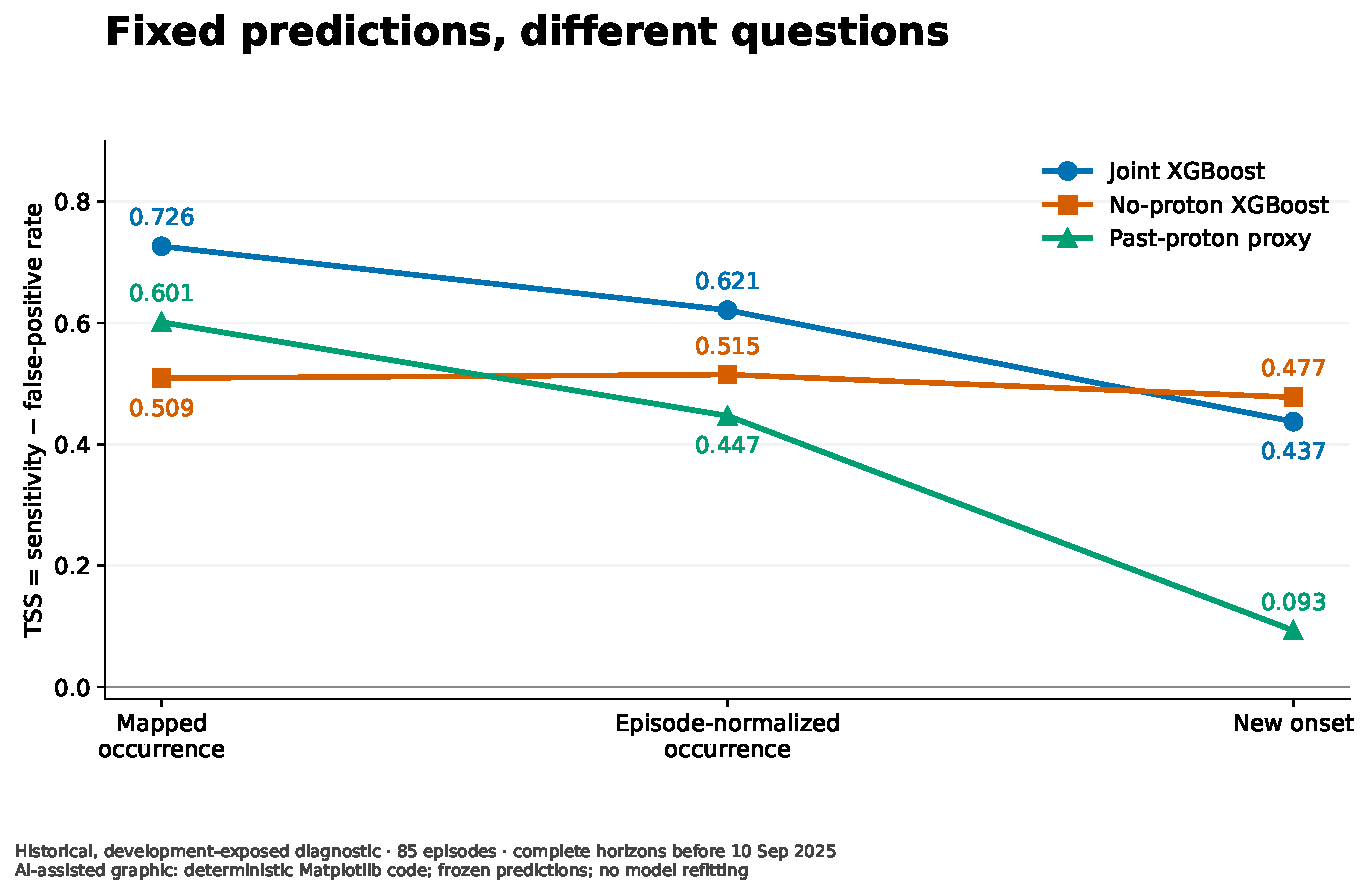
\includegraphics[width=0.92\textwidth]{../audit_20260915/figures/01_fixed_predictions.pdf}
\caption{Fixed predictions under three evaluation views. The lines show changes in what is being measured, not changes caused by retraining.}
\end{figure}

\subsection{Why the score changes}

The repository's exact decomposition shows that the 0.289 joint-XGBoost decrease can be separated into two parts:

\begin{itemize}
    \item \textbf{Multiplicity contribution:} 0.105. Longer episodes receive more rows in ordinary evaluation and are, on average, easier for this model to detect.
    \item \textbf{Persistence contribution:} 0.184. Windows after the event has already started are easier to alert than the true onset window.
\end{itemize}

Therefore,
\begin{equation}
    0.105 + 0.184 \approx 0.289,
\end{equation}
matching the observed mapped-to-onset TSS difference to numerical precision.

This simple decomposition is useful because it distinguishes two effects that would otherwise be mixed together: \emph{how often a storm is counted} and \emph{whether the forecast is being asked to predict a new storm or recognize one already underway}.

\begin{figure}[H]
\centering
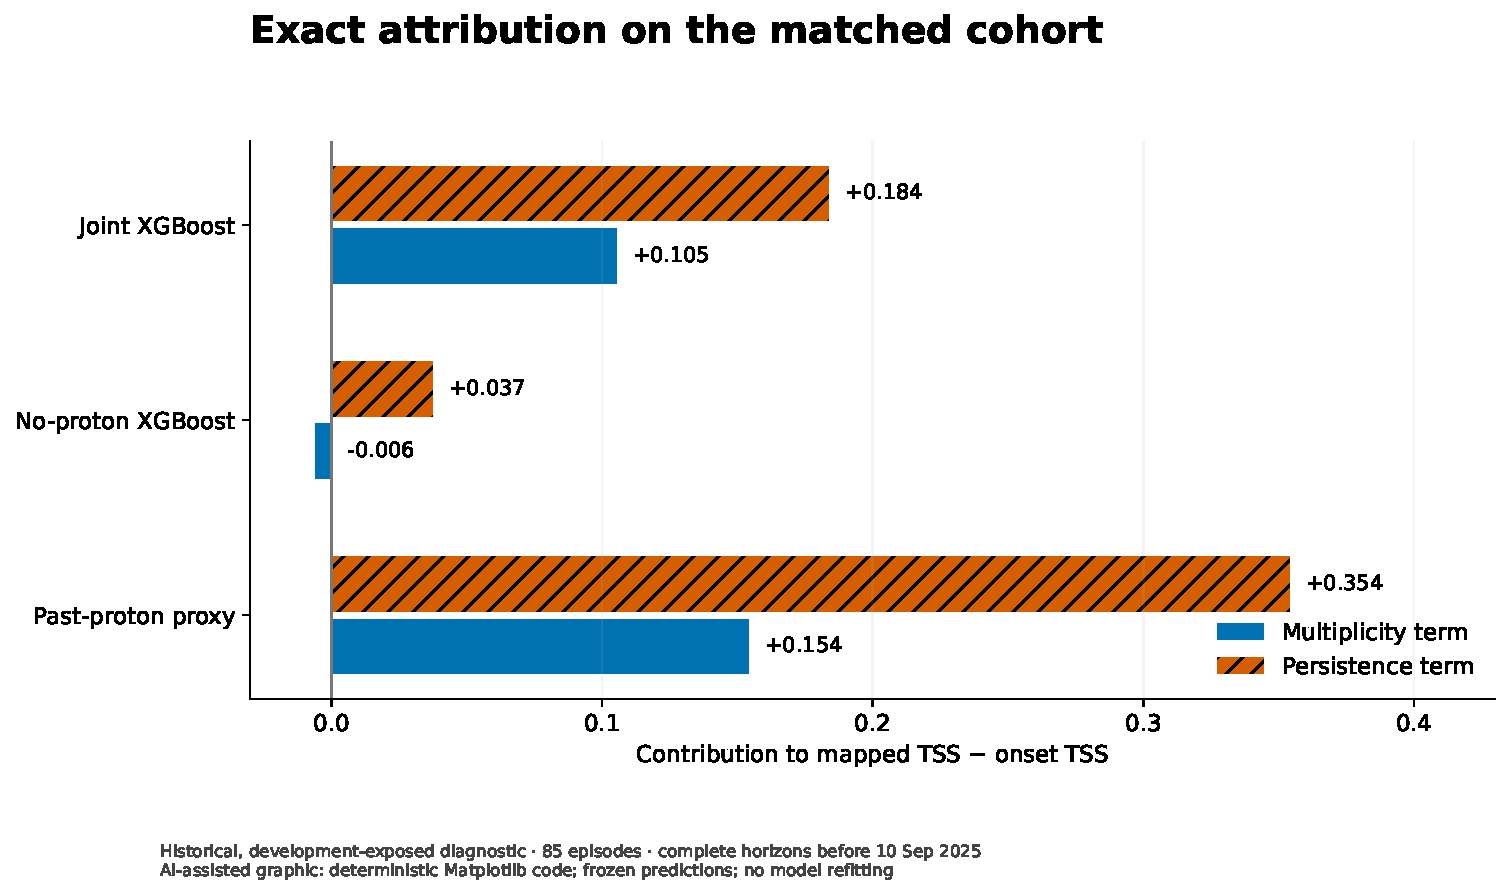
\includegraphics[width=0.92\textwidth]{../audit_20260915/figures/02_decomposition.pdf}
\caption{Measured contributions to the mapped-to-onset score difference. The decomposition explains the fixed historical predictions; it does not prove a causal role for one sensor family.}
\end{figure}

\subsection{The past-proton proxy shows the strongest persistence effect}

The simple past-proton proxy falls from TSS 0.601 in mapped occurrence to 0.093 for new onset. Its total decrease is about 0.508. This is physically plausible: if proton flux was already high in the recent past, it is strong evidence that the same radiation episode may still be active, but it is much weaker evidence for a new first crossing.

This result is useful as a mechanism check. It shows that a predictor can look effective for continuing radiation exposure without being an effective new-storm warning system.

\subsection{No-proton XGBoost is less sensitive to the evaluation change}

The no-proton XGBoost comparator changes only from TSS 0.509 to 0.477 between mapped occurrence and onset. Its pooled episode-normalization change is close to zero. This is consistent with the idea that explicit proton history contributes to persistence recognition.

However, this is not enough to claim that proton features \emph{cause} the full score inflation. The no-proton model still contains other measurements correlated with solar-event duration, and its behavior is not identical in every time period.

The point ordering of joint and no-proton XGBoost also reverses under onset evaluation, but the paired onset difference has a 95\% interval that includes zero. Therefore the project does not claim a statistically reliable model-ranking reversal.

\subsection{Bootstrap intervals preserve the main effect}

For the joint XGBoost model, the paired 95\% interval for episode-normalized minus mapped TSS is approximately
\[
[-0.147,-0.064],
\]
and the interval for onset minus episode-normalized TSS is approximately
\[
[-0.245,-0.125].
\]

For the past-proton proxy, the 95\% interval for onset minus mapped TSS is approximately
\[
[-0.568,-0.442].
\]

All three intervals remain below zero.

When nearby episodes are grouped by 27-day, 90-day, quarterly and yearly calendar bins, the signs of these three main contrasts are preserved. This does not prove that solar-cycle conditions are stationary, but it shows that the result is not explained only by treating every nearby event as independent.

\begin{figure}[H]
\centering
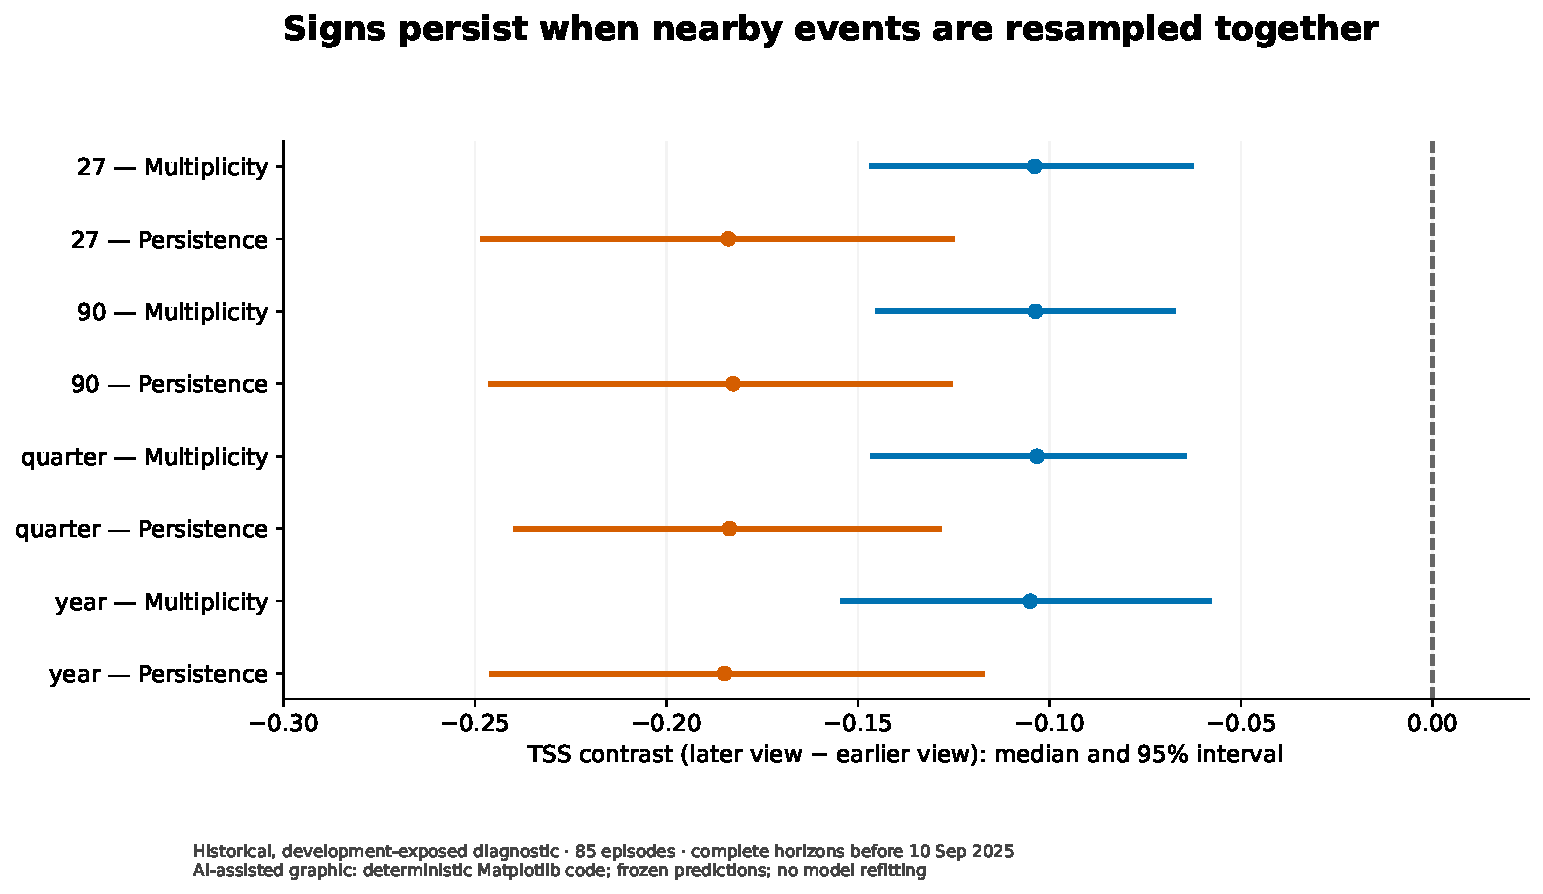
\includegraphics[width=0.92\textwidth]{../audit_20260915/figures/03_temporal_intervals.pdf}
\caption{Temporal-cluster bootstrap checks. Intervals remain on the same side of zero for the three main fixed-prediction contrasts.}
\end{figure}

\subsection{A high TSS does not mean a low false-alert burden}

Under new-onset evaluation, joint XGBoost has TP=41, FN=44, FP=330 and TN=6,982. This gives approximately 48.2\% onset detection, a 4.51\% false-positive rate and an 88.95\% false-alarm ratio.

The difference between FPR and FAR is important. Only a small fraction of negative days are alerted, but because true new onsets are rare, most issued alerts are still false. Therefore the project does not claim that the model is ready for operational deployment.

\section{What each finding is useful for}

\begin{longtable}{p{0.28\textwidth}p{0.34\textwidth}p{0.31\textwidth}}
\caption{Scientific findings and their practical meaning.}\\
\toprule
\textbf{Finding} & \textbf{What it means} & \textbf{Why it is useful} \\
\midrule
\endfirsthead
\toprule
\textbf{Finding} & \textbf{What it means} & \textbf{Why it is useful} \\
\midrule
\endhead
Episode Multiplicity Factor $\approx2.39$ & A represented SEP episode appears in more than one positive daily row on average. & Warns researchers that row count is not the same as physical-event count. \\
\addlinespace
418 persistence vs 228 onset windows in the full audit & Many positive windows occur after an event has already started. & Shows why occurrence forecasting and first-onset forecasting are physically different tasks. \\
\addlinespace
Joint XGBoost TSS $0.726\rightarrow0.621\rightarrow0.437$ & Skill falls even though predictions and thresholds are unchanged. & Demonstrates that the evaluation definition itself can materially change the scientific conclusion. \\
\addlinespace
Multiplicity contribution $\approx0.105$ & Longer episodes are disproportionately represented and easier for the joint model. & Separates event-counting effects from actual onset difficulty. \\
\addlinespace
Persistence contribution $\approx0.184$ & Already-active windows are easier than onset windows for the joint model. & Quantifies how much continuing-storm recognition contributes to the ordinary score. \\
\addlinespace
Past-proton proxy TSS $0.601\rightarrow0.093$ & Recent high proton flux is much better at recognizing continuation than predicting onset. & Provides a physically interpretable mechanism check and a caution against using persistence as proof of early warning. \\
\addlinespace
No-proton XGBoost changes much less & Explicit proton history is associated with stronger evaluation sensitivity, although causality is not proven. & Provides a useful comparator and narrows the physical interpretation. \\
\addlinespace
Temporal bootstrap checks keep the main signs & The result survives several ways of grouping nearby events. & Makes the conclusion more robust to time clustering. \\
\addlinespace
Onset FAR remains very high & Rare-event alerts can still be operationally burdensome even with positive TSS. & Prevents an exaggerated ``deployment-ready'' claim and identifies false-alert reduction as future work. \\
\addlinespace
Direct Phase-II onset model did not validate improvement & A small one-event score period cannot establish a better new-onset forecaster. & Preserves a negative result instead of selecting only favorable experiments. \\
\addlinespace
Separate Phase-II experiment also failed its promotion gate & A later onset-focused design did not reliably beat its regular baseline. & Shows that the project did not rescue the story by repeated model tuning. \\
\addlinespace
Operational-source equivalence remains unresolved & Some historical inputs cannot yet be proven to match what would have been available live. & Prevents retrospective performance from being mislabelled as operational validation. \\
\bottomrule
\end{longtable}

\section{Negative results and research evolution}

A strong part of this project is that failed approaches are retained rather than hidden.

\subsection{Direct onset Phase II}

A direct onset-focused experiment used a 2017 score period containing only one true onset. Its engineered model had TSS about 0.488 compared with 0.411 for an occurrence-trained baseline, but the paired improvement interval included zero. With only one positive event, this does not validate a forecasting improvement.

\subsection{Separate Phase-II experiment}

A separate preregistered experiment contained 3,219 score rows and 21 positives. Its selected two-state/event-weighted model obtained TSS about 0.168 compared with 0.366 for the regular baseline. The improvement interval included zero and the promotion condition failed. This unsuccessful result should remain visible.

\subsection{False-positive controllers}

Two post-processing controllers were tested on the one-event Phase-II probabilities. One reduced false positives but missed the only onset. A second detected the one onset but still produced 50 false alerts, giving a false-alarm ratio of about 98\%. Because the second controller was developed after inspecting the score period, it is a post-hoc development result rather than validation.

\subsection{Operational data-source checks}

The repository also tested whether historical proton science products could be treated as direct equivalents of operational live feeds. Several source contracts failed because energy channels, filenames, sensor orientation or release-time equivalence could not be established. The correct scientific action was to fail closed rather than silently substitute a similar measurement.

These negative findings are useful because they narrow the final claim. The strongest completed contribution is the evaluation study, not a new operational forecast model.

\section{Novelty assessment}

The project contains both known ideas and a potentially original application.

\textbf{Not novel by itself:}
\begin{itemize}
    \item TSS and standard forecast verification;
    \item giving clusters or events different statistical weights;
    \item event-based verification in space-weather science;
    \item the general mathematical fact that weighted averages change when weights correlate with outcomes.
\end{itemize}

\textbf{Potentially novel contribution:}
\begin{itemize}
    \item applying three matched evaluation views to the \emph{same frozen SEP predictions};
    \item explicitly separating repeated physical-event representation from already-active persistence;
    \item quantifying both contributions while keeping the negative cohort fixed;
    \item showing that these changes are large for some SEP predictors but small for others;
    \item preserving negative model-development and live-source results instead of turning them into a model-superiority story.
\end{itemize}

A bounded literature audit did not identify a prior SEP study with this exact combination of fixed predictions, equal-event weighting, onset-only evaluation, matched negatives and explicit attribution. That supports a cautious application-novelty claim. It does \emph{not} justify saying ``first ever'' without a stronger domain-expert literature review.

\section{Scientific and operational significance}

The result is useful because different users may ask different questions.

\begin{itemize}
    \item A spacecraft operator maintaining protection during an existing radiation storm may care about \textbf{occurrence}: will hazardous radiation continue?
    \item A new-warning system may care about \textbf{onset}: will a storm begin within the next 24 hours?
    \item A researcher comparing algorithms may want \textbf{episode-normalized} performance so that one long storm cannot dominate the positive sample simply because it spans many daily windows.
\end{itemize}

The proposed practical change is therefore simple: for window-based SEP forecasting, report all three views when relevant, together with POD, FPR and FAR. This does not replace existing verification; it makes the operational question explicit.

The result may also apply more broadly to rare-event forecasting whenever one physical episode can create repeated positive time windows, for example geomagnetic storms, floods, equipment faults or medical monitoring episodes. Such extensions require separate testing and are not results of the present study.

\section{Limitations}

\begin{enumerate}
    \item \textbf{Historical development exposure.} The central predictions come from public historical data that were available during development. This is not an untouched prospective test.
    \item \textbf{Catalog dependence.} Episode identities and onset windows are defined using the declared event catalog. The complete study has not independently rebuilt every event boundary from raw proton flux.
    \item \textbf{Operational causality.} A variable existing in a modern historical archive does not prove it was available in real time at the original forecast issue time.
    \item \textbf{Model-selection uncertainty.} Bootstrap intervals describe uncertainty in the fixed predictions and sampled physical units. They do not reproduce the whole development process.
    \item \textbf{Solar-cycle change.} Temporal-cluster checks are encouraging but do not establish stationarity across future solar cycles.
    \item \textbf{False-alert burden.} Onset FAR remains high, so the study does not demonstrate deployment readiness.
    \item \textbf{Novelty priority.} The exact application appears underexplored, but a bounded literature search cannot prove universal priority over every SEP paper.
\end{enumerate}

\section{Conclusion}

The main discovery is not a better neural network or a larger headline skill score. It is that the \emph{meaning of the score changes with the physical question being asked}.

In the audited historical cohort, the same joint XGBoost alerts have TSS 0.726 when every positive 24-hour window counts separately, 0.621 when every physical episode receives equal total weight, and 0.437 when only genuine new-onset decisions are evaluated. A simple past-proton rule shows an even larger fall, from 0.601 to 0.093. The score changes occur without model retraining or threshold adjustment.

These results support a practical recommendation: SEP forecasting studies should distinguish continuing-event occurrence, equal-event performance and genuine onset prediction instead of assuming that one window-based score answers all three questions. The current evidence is strong enough for a bounded historical methods study, but not for claims of operational superiority, state-of-the-art forecasting or prospective validation.

\section*{Recommended next experiment}

The highest-value next step is an independently controlled prospective test in which forecasts are timestamped before outcomes are known and the evaluated inputs are proven to have been available at issue time. The same three evaluation views should then be applied without changing the model or thresholds after outcome access. This would test whether the historical evaluation effect generalizes to genuinely unseen future events.

\appendix

\section{Evidence provenance}

The paper scaffold is based on the independent audit overlay at branch head \texttt{c6f05f297165eccc70d298ca40c43e8f6014935d}. Important repository evidence includes:

\begin{itemize}
    \item \texttt{audit\_20260915/PAPER\_RESULTS\_20260920.md}
    \item \texttt{audit\_20260915/AUDIT\_REPORT.md}
    \item \texttt{audit\_20260915/RESULTS\_AND\_EVIDENCE.md}
    \item \texttt{audit\_20260915/MATHEMATICAL\_MECHANISM.md}
    \item \texttt{audit\_20260915/LITERATURE\_AUDIT.md}
    \item \texttt{audit\_20260915/NEGATIVE\_RESULTS.md}
    \item \texttt{audit\_20260915/results/strict\_preboundary\_results.json}
    \item \texttt{audit\_20260915/results/followups\_results.json}
    \item \texttt{tools/audit\_estimands\_v1.py}
\end{itemize}

Frozen replay artifact SHA-256: \texttt{81ec33ee08c89d0e4627e6761fbfa993eccf29e436b6ac32efbfc6f7d954c9b0}.

The audit code verifies that alerts match frozen probabilities and thresholds, checks a common evaluation identity across models, groups positive rows by episode, applies $1/n$ episode weights and preserves the protected-data boundary before interpreting excluded outcomes.

\section{Numbers to understand before defending the project}

\begin{tabularx}{\textwidth}{lX}
\toprule
Number & Meaning \\
\midrule
14,464 & Total daily rows in the full released SEP-PRISM table. \\
650 & Stored positive operational SEP windows in that table. \\
614 / 257 = 2.389 & Uniquely mapped positive windows divided by represented physical episodes. \\
7,509 & Forecast issues in the strict historical diagnostic. \\
197 & Positive windows in the strict diagnostic. \\
85 & Represented onset episodes in the strict diagnostic. \\
0.726 / 0.621 / 0.437 & Joint-XGBoost TSS for mapped, episode-normalized and onset views. \\
0.105 & Joint-model multiplicity contribution. \\
0.184 & Joint-model persistence contribution. \\
0.601 / 0.093 & Past-proton proxy TSS for mapped occurrence / onset. \\
41 / 44 / 330 / 6982 & Joint onset TP / FN / FP / TN. \\
88.95\% & Joint onset false-alarm ratio. \\
4.51\% & Joint onset false-positive rate. \\
10,000 & Number of paired bootstrap draws. \\
\bottomrule
\end{tabularx}

\begin{thebibliography}{9}

\bibitem{whitman2023}
K. Whitman et al.,
``Review of Solar Energetic Particle Prediction Models,''
\emph{Advances in Space Research}, 2023.

\bibitem{balch2008}
C. C. Balch,
``Updated verification of the Space Weather Prediction Center's solar energetic particle prediction model,''
\emph{Space Weather}, vol. 6, 2008.

\bibitem{sepprism2026}
Y. Yu, Y. Chen, L. Zhao, K. Whitman, W. Manchester and T. Gombosi,
``SEP-PRISM Data: A multi-source dataset for solar energetic particle forecasting,''
arXiv:2607.16160, 2026.

\bibitem{sepnet2025}
Y. Yu, Y. Chen, L. Zhao, K. Whitman, W. Manchester and T. Gombosi,
``Solar Energetic Particle Forecasting with Multi-Task Deep Learning: SEPNet,''
arXiv:2512.12786, 2025.

\bibitem{shapelets2025}
``Predicting Solar Energetic Particle Events with Time Series Shapelets,''
\emph{The Astrophysical Journal}, 2025.

\end{thebibliography}

\end{document}
